\documentclass[12pt, preprint]{aastex}
\usepackage{graphicx}	% For figures
\usepackage{natbib}	% For citep and citep
\usepackage{amsmath}	% for \iint
\usepackage{bbm}
\usepackage[breaklinks]{hyperref}	% for blackboard bold numbers
\usepackage{hyperref}
\hypersetup{colorlinks}
\usepackage{color}
\usepackage{morefloats}
\definecolor{darkred}{rgb}{0.5,0,0}
\definecolor{darkgreen}{rgb}{0,0.5,0}
\definecolor{darkblue}{rgb}{0,0,0.5}
\hypersetup{ colorlinks,
linkcolor=darkblue,
filecolor=darkgreen,
urlcolor=darkred,
citecolor=darkblue }


\newcommand{\beq}{\begin{equation}}
\newcommand{\eeq}{\end{equation}}

\begin{document}
\title{Fast and optimal centroiding of faint stars}

\author{
  Mohammadjavad~Vakili\altaffilmark{1},
  David~W.~Hogg\altaffilmark{1,2,3}}
\altaffiltext{1}{Center for Cosmology and Particle Physics, Department of Phyics,
             New York University, 4 Washington Pl., room 424, New York, NY, 10003, USA}
\altaffiltext{2}{Center for Data Science, New York University, 726 Broadway, 7th Floor, New York, NY 10003, USA}
\altaffiltext{3}{Max-Planck-Institut f\"ur Astronomie, K\"onigstuhl 17, D-69117 Heidelberg, Germany}
\email{mjvakili@nyu.edu}


\begin{abstract}
One of the most demanding tasks in astronomical image processing---in terms of precision---is measurement
of the positions of stars. 
Upcoming ground-based surveys are going to take images of billions of point sources, 
including many faint stars, with short exposure times. Real-time estimation of the
centroids of stars is crucial for real-time PSF estimation, and maximal precision is required
for measurements of proper motion. In this work, we aim to compare the performance of
various centroiding methods, when they are applied
to relatively low signal-to-noise ratio unsaturated stars.
In order to investigate how information-preserving these techniques are, we compare
the root-mean-squared-error with the fundamental Cramer-Rao
bound on precision. We discuss the case in which we have a good estimate
of the PSF, and the case in which we don't. In the first case, we show that a fast
 polynomial centroiding after smoothing the image by the PSF can be 
as accurate as full PSF profile fitting. In the second case, we demonstrate 
that although polynomial centroiding is not as
accurate as PSF profile fitting, it comes close to saturating the Cramer-Rao bound
in a wide range of conditions. We also show that the center-of-light (or the taking of moments) 
never comes close to saturating the bound.
\end{abstract}

\section{Introduction}

When we take imaging---and we take prodigious amounts of imaging---we ususally have to find the coordinates
of the stars in that imaging. Finding accuarate estimates of the centers of point
sources, convolved with telescope point spread function (and atmospheric PSF in the case of
ground-based telescopes), and also pixel response function, is usually crucial to all further steps in the 
image processing pipeline. For instance, proper measurement of the shapes of galaxies
requires interpolating the PSF from the positions of sparsely located stars across the
image to the positions of galaxies. The accuracy of the PSF estimation therefore,
relies on how accurately we know the centroids of stars. 

Ideally, we want a centroiding procedure that provides measurements as accurate as possible,
without putting a huge computational burden on the photometric pipeline.
Reducing the computational cost becomes even more important in large surveys,
where we want to estimate the centroids of many thousands of point sources detected
on the telescope's focal plane in real time. 

Measurement of the centroids of stars however, is limited
by lack of knowledge about the exact shape of the PSF, and also the presence of noise;
both sky noise and CCD readout noise. Thus, it is of particular interest to devise a fast method that returns
optimal estimates of centroids in a realistic range of signal-to-noise ratios.

To date, a number of software packages have been designed for the purpose of extracting astronomical
sources and making catalogs. One of these softwares is \textsl{SExtractor} \citep{sex},
whose centroiding method involves first, finding the zeroth moment of the object
as a first-order estimate, and then iteratively correcting the centroid by computing
the zeroth order moment of the object weighted by a Gaussian window function,
until the correction falls below a particular threshold value.
The width of the Gaussian window function is set by the object's half-light radius.

Other examples are DAOPHOT \citep{daophot}, and DOPHOT \citep{dophot}
which both assume analytic models for the stellar PSF profiles with centroid
coordinates being free parameters of these models.
DAOPHOT (DoPHOT) finds the centroids by fitting a Gaussian (truncated power series for a Gaussian) PSF to
the light profile of stars.

In this paper, we compare various techniques for centroiding 
faint unsaturated stars. That is, we apply a number of centroiding methods 
to a large number of simulated faint stars with different signal-to-noise ratio and
 size realizations. Uncertainties from star centroiding methods will always have 
a theoretically-set lower bound, known as the Cramer-Rao lower bound
(hereafter denoted by CRLB), which has an inverse relation with the
signal-to-noise-ratio of stars (see section \ref{sec:CRLB}).

Given the analytic expression for the PSF model,
we derive an expression for the fundamental lower bound on the centroiding error as
a function of the parameters of the PSF model (\eg size),
and signal-to-noise-ratio of stars. We create two sets of simulations for which we 
know the CRLB, one with variable (constant) signal-to-noise ratio (FWHM), and one 
with variable (constant) FWHM (signal-to-noise ratio). After applying
different centroiding methods to the simulations,
we investigate how close these methods can get to saturating the CRLB for
various ranges of background noise level and PSF FWHM.
%%%%%%%%%%%%%%%%%%%% FIXED%%%%%%%%%%%%%%%%%%%
In this work, we focus on four centroiding methods. The first method
involves fitting a PSF profile, assuming that we have a good PSF estimate, to the star. 
The second method estimates the centroid of a star by convolving the image with the PSF 
and then fitting a 2d second-order polynomial to
 the 3$\times$3 patch around the brightest pixel. The third method centroids stars by
 smoothing the image of stars with a Gaussian kernel of a fixed size,
 and then applying the same 3$\times$3 polynomial fit to the smooth
 image. This method is fast and does not require any knowledge of the 
PSF. The last method we consider, the center of light centroiding, involves computing moments in the
 7$\times$7 patch centered at the brightest pixel of the image.
%%%%%%%%%%%%%%%%%%%%%%%%%%%%%%%%%%%%%%%%%%%%%%%%%%%%%%%%%%%
This paper is structured as follows. In section \ref{sec:CRLB},
we discuss the Cramer-Rao lower bound, and we derive
an analytic expression for the lower bound on centroiding error
of the simulated data, and also PSF profile fitting. 
In section \ref{sec:method} we give a brief overview of approximate 
centroiding methods used in our investigation.
In section \ref{sec:data} we discuss the Cramer-Rao lower bound satuaration
tests and their corresponding simulated data.
In section \ref{sec:result}, we compare the performances of the methods
discussed in \ref{sec:method}, with the CRLB derived in \ref{sec:data}. Finally,
 we discuss and conclude in \ref{sec:discussion}.               
%%%%%%%%%%%%%%%%%%%%%%%%%%%%%%%%%%%%%%%%%%%%%%%%%%%%%%%%%%%%%%%%%%%% Cramer-Rao lower Bound %%%%%%%%%%%%%%%%%%%%%%%%%%%%%%%%%%%%%%%%%%%%%%%%%%%%%%%%%%%%%%%%%%%%%%%%%%

\section{Cramer-Rao lower bound on centroiding error}\label{sec:CRLB}

In order to test the accuracy of various centroiding methods, we need to to compare their 
performances against each other at saturating the Cramer-Rao lower bound on centroiding error. 
The closer an estimator is to saturating 
the CRLB, the more information about the quantity that we 
need to estimate is preserved. A measure for closeness of an estimator to 
saturating the CRLB is comparison of the root-mean-squared-error of that estimator 
with the CRLB. 

The CRLB is given by the inverse of 
the Fisher information matrix $\mathcal{F}$. Thus, in order to find the CRLB,
 it is sufficient to compute the Fisher matrix.
 
Let us assume that there are $M$ observables $\{f_{1}, ... , f_{M}\}$, each
related to $B$ model parameters $\{\theta_{1} , ... , \theta_{B}\}$
\beq
f_{m} = f_{m}(\theta_{1} , ... , \theta_{B}) \,\, m=1,...,M
\eeq
Assuming
uncorrelated Gaussian error $\sigma_{m}$ for each observable $f_{m}$, elements
of the Fisher matrix $\mathcal{F}_{ij}$ are given by
\beq
\mathcal{F}_{ij} = \sum_{m}\frac{1}{\sigma_{m}^{2}}\frac{\partial f_{m}}{\partial \theta_{i}}\frac{\partial f_{m}}{\partial \theta_{j}}
\label{fisher}
\eeq

This requires simulation of a large set of stars for which we know the exact position of centroids
and the corresponding lower bound for each star, and comparing the centroiding error with the lower bound.



%%%%%%%%%%%%%%%%%%%%%%%%%%%%%%%%%%%%%%%%%%%%%%%%%%%%%%%%%%%%%%%% THIS GOES TO TESTS%%%%%%%%%%%%%%%%%%%%%%%%%%%%%%
%Furthermore, we uniformly draw the centroids of these simulated stars within sub-pixel regions. 
%We aim to study how centroiding errors from different methods behave with
%changing SNR and size, and how close they get to saturating the CRLB. 
%%%%%%%%%%%%%%%%%%%%%%%%%%%%%%%%%%%%%%%%%%%%%%%%%%%%%%%%%%%%%%%%%%%%%%%%%%%%%%%%%%%%%%%%%%%

We use the Moffat profile \citep{moffat} for our PSF simulations. 
Moffat profile is an analytic model for stellar PSFs. It has broader wings than
a simple Gaussian profile. The surface brightness of the Moffat profile is given by
\beq
I(r) = \frac{F(\beta -1)}{\pi \alpha^{2}}[1+(r/\alpha)^{2}]^{-\beta},
\label{mof}
\eeq
where $F$ is the total flux, $\beta$ is a dimensionless paramter, and $\alpha$ is
the length scale of the Moffat profile, with FWHM (hereafter denoted by $\gamma$)
being $2\alpha\sqrt{2^{1/\beta}-1}$. 
We aim to investigate the performance of centroiding methods for
 different background noise levels, and also different
values of $\gamma$. For further simplicity, we set the flux of all stars in our
simulations to unity. Per pixel uncertainties are assumed to be uncorrelated Gaussian,
and we only study the sky-dominated regime.

Moreover, it is more convenient to work with the signal-to-noise ratio
(hereafter denoted by SNR) instead of the variance of the Gaussian noise.
We use the definition of SNR according to which, SNR is given by the ratio
 of the mean and variance of the distribution
which the flux estimator is drawn from. Assume that the total flux from
the point source is $F$, and that the PSF at the $i$-th pixel is given
by $P_{i}$. Therefore the brightness of the $i$-th pixel is drawn from
a Gaussian distribution $p(I_{i}) = \mathcal{N}(FP_{i},\sigma^{2})$. 

The optimal estimator of flux (one that saturates Cramer-Rao bound),
is the weighted average $\tilde{F}=\sum_{i}y_{i}P_{i}$. Knowing the
distribution of $I_{i}$, it can be shown that 
\beq
p(\tilde{F}) = \mathcal{N}(F , \frac{\sigma^{2}}{\sum_{i}P_{i}^{2}}),
\eeq  
which leads us to
\beq
\begin{array}{l}
\text{SNR} $=$ \frac{\sqrt{\sum_{i} P_{i}^{2}}}{\sigma}.
\end{array}
\label{snr}
\eeq

Note that (\ref{snr}) is valid in the limit of sky-dominated regimes,
and that is the limit we are interested in throughout our investigation.
 In the case of Moffat profiles, SNR given in (\ref{snr}) can be analytically 
expressed in terms of the per pixel uncertainty
$\sigma$, FWHM $\gamma$, and also $\beta$. We hold $\beta$ fixed at the fiducial value of 2.5.
In this case we have
\beq
\text{SNR} = \frac{0.478}{\sigma \gamma}.
\label{snr2}
\eeq

Equation (\ref{snr2}) implies that for stars with the same flux $F$,
 and background
noise level $\sigma$, those with higher size have lower SNR.

Given the PSF model that we have adopted for our simulations, we can derive
 an expression for the CRLB as a function of the size, and SNR of stars.
 
In our case, the observables are Moffat PSF profile evaluated at different pixels, and  
the model paramters are the centroid coordinates. Thus, $\mathcal{F}$
is a 2$\times$2 matrix whose elements are given by

\beq
  \mathcal{F}_{ij} = \sum_{\mathbf{p}}\frac{1}{\sigma_{\mathbf{p}}^{2}}
                \frac{\partial f_{\mathbf{p}}}{\partial \theta_{i}}\frac{\partial f_{\mathbf{p}}}{\partial \theta_{j}},
\label{fish}
\eeq
where the summation is over pixels, $f_{\mathbf{p}}$ is the value of the Moffat profile at pixel $\mathbf{p}$,
$\theta=\{x_{c},y_{c}\}$, $\sigma_{\mathbf{p}}^{2}$ is variance
of the uncorrelated Gaussian noise map $n(\mathbf{x_{p}})$
\begin{eqnarray}
\langle n(\mathbf{x_{p}}) \rangle &=& 0, \\
\langle n(\mathbf{x_{p}})n(\mathbf{x_{p^{\prime}}}) \rangle &=& \sigma^{2}\delta_{\mathbf{p}\mathbf{p}^{\prime}}. 
\end{eqnarray}

Given the analytic expression for the Moffat PSF model (\ref{mof}), and choice of $\beta=2.5$, 
the inverse of the Fisher matrix is given by
\beq
  \mathcal{F}^{-1} \simeq 0.6846 \frac{\gamma}{\text{SNR}} 
  \begin{pmatrix}
      1 & 0\\
      0 & 1\\
  \end{pmatrix}.
\label{crlbmoffat}
\eeq

Equation (\ref{crlbmoffat}) implies that at given SNR and $\gamma$,
CRLB for each component of centroid is given by $0.6846\gamma/\text{SNR}$,
and that a good centroiding technique delivers centroids with
root-mean-squared-error (hereafter RMSE) of each component close to
this number.

%%%%%%%%%%%%%%%%%%%%%%%%%%%%%%%%%%%%%%%%%%%%%%%%%%%%%%%%%%%%SAY SOMETHING MAARRRR%%%%%%%%%%%%%%%%%%%%%%%%%%%%%%%%%%%%%%%%%%%%
We examine fitting an exact
 PSF profile to the stars. That is, in our Cramer-Rao bound saturation tests, we find the best
 estimates of flux and centroid by optimizing the $\chi^{2}$.
 We expect this method to perform better in determing the centroids
 of stars. In theory, this method should always saturate the CRLB. 
  
\section{Approximate methods}\label{sec:method}

\item{\bf  PSF-based 3$\times$3 polynomial centroiding}\quad Let us consider the case 
in which we have a good estimate of the PSF at
the position of the faint star under consideration. 
We can smooth the image of the star, by convolving it with the 
full postage stamp of the PSF. Then, we fit a simple 2d polynomial 
$P(x,y)=a+bx+cy+dx^2+exy+fy^2$ 
to the 3$\times$3 patch around the brightest pixel of the convolved image.
Upon constructing a universal 9$\times$6 design matrix
\begin{equation}
    \mathbf{A} = 
    \begin{bmatrix}
        1 & x_{1} & y_{1} & x_{1}^{2} & x_{1}y_{1} & y_{1}^{2} \\
        . & . & . & . & . & .  \\
        . & . & . & . & . & .  \\
        . & . & . & . & . & .  \\
        1 & x_{9} & y_{9} & x_{9}^{2} & x_{9}y_{9} & y_{9}^{2}
    \end{bmatrix},
\end{equation}
the free parameters $\{a,b,c,d,e,f\}$
(hereafter compactly denoted by $\mathbf{X}$) can be determined by 
\beq
\mathbf{X} = (\mathbf{A}^{T}\mathbf{A})^{-1}\mathbf{A}^{T}\mathbf{Z},
\label{linearfit}
\eeq
where $\mathbf{Z}$ is given by $(z_{1},...,z_{9})^{T}$,
with $z_{i}$, being the brightness of the $i-$th pixel of the 3$\times$3 patch.
Afterwards, the best fit parameters can be used to compute the centroid coordinate

\beq
  \begin{bmatrix}
      x_{c}\\
      y_{c}\\
  \end{bmatrix} = 
  \begin{bmatrix}
      2d & e\\
      e & 2f\\
  \end{bmatrix}^{-1}
  \begin{bmatrix}
      -b\\
      -c\\
  \end{bmatrix}.
\label{center}
\eeq

It is important to note that the algebraic operation in (\ref{center}) involves 
inverting a 2$\times$2 curvature matrix
\beq
  D = 
  \begin{bmatrix}
      2d & e\\
      e & 2f\\
  \end{bmatrix}.
\eeq

When $D$ has a zero (or very close to zero) deteminant,
centroid estimated by (\ref{center}) gets arbitrarily 
large in which case the centroiding method leads to a catastrophic 
outlier. In order to tackle this issue, we add a soft regularization term
proportional to $\sigma^{2}$ to the determinant of $D$.

The procedure of convolving the image of star with the PSF results in a
more well-sampled image, which eventually, leads to having more
information regarding the centroids of stars in the 3$\times$3 patch around the
brightest pixel. In addition, a simple 2d polynomial will provide a better fit 
since convolution with the PSF makes the variation of the brightness of the image
 across the 3$\times$3 patch very smooth.
 
\item{\bf 3$\times$3 polynomial centroiding}\quad In the case that 
we do not have know the PSF at the position of star, we change 
the smoothing step in the following way. Instead of smoothing the image 
with the PSF, we smooth it with a Gaussian kernel of a fixed size. 
\beq
k(\mathbf{x}) = \frac{1}{2\pi w^2}\exp(-\mathbf{x}^{2}/2w^{2}).
\eeq
Throughout this study, the full-width at half-maximum of the Gaussian kernel is held at
a fixed value of 2.8 pixels (corresponding to w $\simeq$ 1.2 pixels).

Then we apply the same 2d polynomial method to the 3$\times$3 patch around the brightest
pixel of the smoothed image. Therefore, for a given star and a smoothing kernel,
the outcome of equation (\ref{linearfit}) can be
plugged into equation (\ref{center}) to find the centroid estimate
of the star. This is inspired by the 3$\times$3 quartic approximation 
used in the \textsl{Sloan Digital Sky Surveys} photometric pipeline \citep{sdss}.

\item {\bf Center of light centroiding}\quad In addition to the methods 
mentioned so far, we examine centroiding stars by computing their zeroth moments
in a 7$\times$7 patch around the brightest pixel of the image.
In terms of saturating the Cramer-Rao lower bound, we expect this simple 
center of light centroiding to perform worse than all other methods mentioned in 
this section. Hereafter, we call this method $7\times7$ moment centroiding.

%%%%%%%%%%%%%%%%%%%%%%%%%%%%%%%%%%%%%%%%%%%%%%%%%%%%%%%%%%%%%%%%%%%%THIS METHOD SUCKS BALLS%%%%%%%%%%%%%%%%%%%%%%%

\section{Tests}\label{sec:data}

We perform two sets of simulations. In the first set, we choose four values of
2, 2.8, 4, and 5.6 pixels for $\gamma$. For each $\gamma$, we generate 100,000 
17 $\times$ 17 postage-stamps of Moffat profiles with centroids randomly drawn
within the central pixel of the 17 $\times$ 17 postage-stamps. Moreover, Gaussian
noise is added to each postage-stamp such that the simulated stars are uniformly
 distributed in log-SNR between SNR = 5 to SNR = 100.

In the second set, we generate 100,000 17$\times$17 postage-stamps
of Moffat profile, with values of $\gamma$ uniformly distributed 
between 2 and 6 pixels, and with centroids drawn randomly within 
the central pixel. We choose four values for SNR: 5, 10, 20, and 40. 
For each SNR, and for each postage-stamp with a given $\gamma$, 
Gaussian noise, with variance corresponding to SNR and $\gamma$ through equation 
(\ref{snr2}), is added to each postage-stamp.

In the first experiment, we study how centroiding error behaves with changing
SNR, while $\gamma$ is held constant. In the second experiment, we study 
how centroiding error behaves with changing $\gamma$ while SNR is held constant.

\section{Results}\label{sec:result}

\subsection{Experiment 1}
   
In this experiment, after finding the centroiding error for each method,
we compute the RMSE in bins of SNR in order to compare it to the CRLB. 
Results of the first experiment are shown in Figures [\ref{1}], [\ref{2}],
[\ref{3}], [\ref{4}]. All methods deliver results with RMSE larger 
for fainter stars.

As we expected, the RMSE from centroiding by fitting the exact PSF model [\ref{1}]
lies on the CRLB except for simulations with SNR $\la$ 10 where the RMSE gets slightly pulled away
from the CRLB due to presence of a few outliers. Figure [\ref{2}] demonstrates that even the PSF-based 3$\times$3 polynomial 
centroiding is able deliver centroiding estimates as accurate as PSF profile fitting, with the exception
of simulated stars with $\gamma$ = 2 pixels. For stars with $\gamma$ = 2 pixels, although the 3$\times$3 polynomial
fitting gets close to saturating the CRLB, it fails to saturate the CRLB since the PSF is undersampled. For simulated images with higher $\gamma$, convolving the
data with the PSF result in images that are well-sampled around the brightest pixel. This allows the 
polynomial centroiding to deliver highly accurate results that can saturate the CRLB for simulated
data with SNR $\ga$ 10.

RMSE from the 3$\times$3 polynomial centroiding [\ref{3}],
is very close to the CRLB except at the very small values of SNR (SNR $\la$ 10).
As we increase $\gamma$ from 2 pixels to 2.8 pixels, RMSE gets closer
to the CRLB. When we increase $\gamma$ to
4 and 5.6 pixels, RMSE gets farther from the CRLB. For stars with $\gamma$ = 2 pixels, 
the rate at which the RMSE from this method drops
eventually becomes smaller than the constant rate at which the CRLB
decreases with increaing SNR. The reason for this is that even after smoothing
the with a Gaussian kernel, the image is still relatively undersampled, and not smooth enough
for a 2d polynomial fitting to provide highly accurate centroiding estimates.
For stars with $\gamma=2.8$ pixels, since the FWHM of the Gaussian kernel matches that 
of the PSF of underlying simulations, the smooth images are well-sampled and therefore, 
the method is able to deliver estimates extremely close to saturating the CRLB. As $\gamma$
gets higher for the simulations, the convolved images are not as well-sampled as those 
whose $\gamma$ matches the FWHM of the smoothing kernel and as a result, we loose
some information by fitting a polynomial to a 3$\times$3 patch. Therefore,
 we observe slight deviation from the CRLB for stars with $\gamma$ = 4 pixels, and 
slightly more deviation as we increase $\gamma$ to 5.6 pixels.

However, in case of 7$\times$7 moment method [\ref{4}], RMSE becomes
quite large as we move towards fainter stars in our simulation.
For stars with larger $\gamma$, centroid estimates from the naive center of light 
centroiding show large deviation from saturating the CRLB. By increasing $\gamma$,
RMSE deviates further away from the CRLB.

\subsection{Experiment 2}

In this experiment, after finding the centroiding error for each method, we
compute the RMSE in bins of $\gamma$ in order to compare it to the CRLB. 
Behavior of error as a function of $\gamma$ for different values of SNR,
is shown in figures [\ref{5}], [\ref{6}], [\ref{7}], and [\ref{8}]. 
 
Once again, the RMSE from centroiding by fitting the exact PSF model as a function of FWHM
perfectly lies on the CRLB except at SNR = 5 where the RMSE slightly deviates
from the CRLB due to presence of a few outliers [\ref{5}]. 
Thus, centroid estimates from fitting
the exact PSF model always saturate the CRLB. Once again, we observe that the centroid
estimates found by the PSF-based 3$\times$3 polynomial centroiding saturate the CRLB with the
exception of simulated stars with SNR = 5, or $\gamma$ very close to 2 pixels [\ref{6}].

The 3$\times$3 polynomial method [\ref{7}], results in RMSE very close to the CRLB.
For all four values of SNR, as we increase $\gamma$ from 2 pixels to 3 pixels,
RMSE gets slightly closer to the CRLB since the method starts to perform
slightly better as we move away from undersampled stars, and as the FWHM of the smoothing kernel
gets closer to that of the simulated images.
After approximately 3 pixels, increasing $\gamma$ result in deviation of RMSE of the method from the CRLB.
This is a characteristic of 3$\times$3 method as we apply it to a smoothed image which is still not sufficiently
well-sampled.  Furthermore, increasing SNR from 5 to 40 makes the RMSE (as a function of $\gamma$) become
closer to the CRLB.

The centroid estimates obtained from the naive 7$\times$7 moment method [\ref{8}]
result in RMSE much larger than the CRLB in all ranges of FWHM and for all four
values of SNR in this experiment. In the case of extremely faint stars (SNR = 5),
the polynomial method is not able to deliver any reliable estimate, and completely fails.

\section{Discussion}\label{sec:discussion}

An optimal stellar centroiding algorithm must saturate the fundamental Cramer-Rao lower 
bound. That is, in all ranges of background noise level, size, radial light profile,
and shape, it must preserve information about the centroids of stars. In practice however,
this is only achievable when we have a reasonably good estimate of the PSF. Since, we do not always 
know the exact PSF profile, we make use of various approximate centroiding algorithms. In this work, we
studied how different methods come close to saturating the CRLB for relatively low signal-to-noise ratio
unsaturated stars.
 
We focused on examples from two classes of centroiding algorithms. The first class contains fast and approximate
methods that do not require any knowledge of the PSF at the positions of stars. Of methods that belong to this class,
we consider centroiding stars based on fitting a low order
polynomial to a 3$\times$3 patch of star images smoothed by a Gaussian kernel of fixed width, and finding the center of light 
of a 7$\times$7 patch around the brightest pixel of the star.
The second class of centroiding algorithms contains methods that require knowledge of the PSF (or having a good estimate
of the PSF) at the positions of stars. We considered two examples from this class. The first example
is the 3$\times$3 polynomial centroiding applied to the image of the star convolved with the PSF, and the
second example is the full PSF profile fitting. In terms of saturating the Cramer-Rao bound, we compared 
the performances of these methods against each other.

%Furthermore, we compared the performance of these methods with the naive 3$\times$3 polynomial
%centroiding, 3$\times$3 quartic approximation, moment-based method, and PSF fitting.
%In order to make this comparison, we performed some tests on a large number of
%simulated data, and investigated to see if these estimators can saturate the Cramer-Rao
%lower bound, or how close to they get to saturating the bound.
 
Our results suggest that in all ranges of FWHM and SNR, the PSF fitting method returns 
centroid estimates that saturate the CRLB; with the exception of SNR being less than 10, 
in which case a few centroiding ouliers caused the RMSE to slightly, but not significantly, deviate
from the CRLB. We found that the estimates found by 7$\times$7 moment method, except in the case of
very high SNR values and very small ranges of $\gamma$, do not come close to
saturating the CRLB. In a considerable range of PSF sizes and background noise levels, 
this method completely fails to deliver any reliable centroiding estimates.
 
On the other hand, the RMSE of centroid estimates of 
3$\times$3 polynomial centroiding are much closer to saturating the CRLB in all ranges of signal-to-noise ratio.
The performance of this method however, is limited by
two important factors: \emph{(i)} signal-to-noise ratio, and \emph{(ii)} PSF size.
The 3$\times$3 polynomial centroiding technique only takes advantage of the information
 contained in a 3$\times$3 patch around the brighest pixel of the smoothed image which is only
 well-sampled when the FWHM of the simulated image of star
 matches that of the smoothing kernel. Thus, when we apply 
this method to find the centroid of stars with larger FWHM, certain amount of
information (encoded in the Cramer-Rao lower bound) is lost, and therefore, the RMSE
of these methods deviates from the CRLB. This deviation becomes even larger at lower
signal-to-noise ratios. Besides, the performance of this method slightly degrades
in the case of undersampled stars (with FWHM close two 2 pixels). 
Presence of noise is another limitting factor.
Although this method is able to get very close to saturating the CRLB in a wide range of
signal-to-noise ratios, it is not reliable in the case of extremely faint stars.
 This is partly due to the fact that in the presence of noise, 
the brightest pixel of image does not necessarily contain the centroid of stars even after smoothing 
the image.

Once we modify the polynomial method further by smoothing the image with the full postage stamp
of the PSF, we obtain results that saturate the CRLB in a wide range of PSF sizes and noise levels.  
This is due to the fact that once the images are convolved with the correct PSF, they become so well-sampled and smooth
that fitting a 2d polynomial to the 3$\times$3 patch around the brightest pixel of the smooth image is sufficient for us to obtain
results as accurate as those from fitting a PSF profile. The only conditions in which slight deviation from
saturating the CRLB occures are very low signal-to-noise ratios (SNR $\la$ 10), and undersampled PSF (FWHM $\sim$ 2 pixels).
One advantage of this method over PSF fitting method is that it is fast, and that it is able to saturate the CRLB in 
a wide range of conditions. In the case that we have a good estimate of the PSF, the 
PSF-based 3$\times$3 polynomial centroiding is a significantly much faster algorithm. 
Although this method is more accurate than 3$\times$3 polynomial centroiding, it is
slightly slower because it requires convolution of the image with the full potage stamp of the PSF. 

In this investigation we showed that PSF fitting is always better at centroiding stars.
However, this method has its own disadvantages. First, we do not always know the the exact PSF. Second, finding
 the centroid by profile fitting is computationally expensive, whereas by employing any of the 3$\times$3 polynomial techniques 
considered in this study into large scale astronomical surveys can considerably reduce the computational cost
of initial astrometry of the point sources detected by these surveys. 

Moreover, it is important to note that the PSF fitting method can be made faster by only keeping the 
term proportional to the dot product of the PSF model and the image in $\chi^2$. This is because 
the other terms in $\chi^{2}$ are not sensitive to the position of the centroid. However, this only allows
us to vary the poition of centroid, and not the flux, while fitting the PSF model
to the star. 

Modifying the $\chi^2$ such that it contains the dot product of the PSF and image, 
provides a nice interpretation for the PSF fitting method. It corresponds to searching for the 
centroid in a very high resolution grid which the dot product of the image and the PSF model is
sensitive to. On the other hand, one can think of the initial smoothing step in the 3$\times$3 polynomial method 
as upsampling of the image around the center through convolving it with an approximate Gaussian PSF. 
The PSF profile fitting and the 3$\times$3 polynomial centroiding are different in that when there is mismatch between the
widths of the smoothing kernel and the that of the PSF, we loose some information by employing a 3$\times$3 polynomial trick.
When we have the advantage of knowing the PSF, this issue can be resolved by employing the PSF-based polynomial method.

Having a reasonable PSF model always helps us obtain more reliable centroid estimates, but
over a certain range of low signal-to-noise ratios and PSF sizes, one can achieve sensibly
 accurate results by employing a simple 3$\times$3 method after smooting the image with
 a Gaussian kernel of fixed width, and without making any assumption about the PSF model.

In this investigation we narrowed our focus on a set of data simulated from a particular
PSF profile. Although there are various cases where Moffat profiles provide reasonable
representations of point spread function, these profiles are not generic enough to let us
reach a more general conclusion. Another important, and untapped, area of study
would be devising a model that infers the centroids of stars and point spread function
(in its full extent, not at the catalog level) across an astronomical image simultaneously.
This is beyond the scope of this study. 


\begin{thebibliography}{70}

\bibitem[Bertin \& Arnouts (1996)]{sex} Bertin, E., Arnouts, S. \ 1996  Astronomy and Astrophysics Supplement Series, 117, 393-404
\bibitem[Lupton etal. (2001)]{sdss} Lupton, R. etal. \ 2001  arXiv: astro-ph/0101420
\bibitem[Schechter etal. (1993)]{dophot} Schechter, P. L., Mateo, M., Saha, A. \ 1993 \pasp, 1342-1353
\bibitem[Stetson (1987)]{daophot} Stetson, P. B. \ 1987, \pasp, 191-222
\bibitem[Trujillo etal. (2001)]{moffat} Trujillo, I., et al. \ 2001 \mnras, 977-985

\end{thebibliography}

\clearpage

\begin{figure}[!htb]
\minipage{.8\textwidth}
  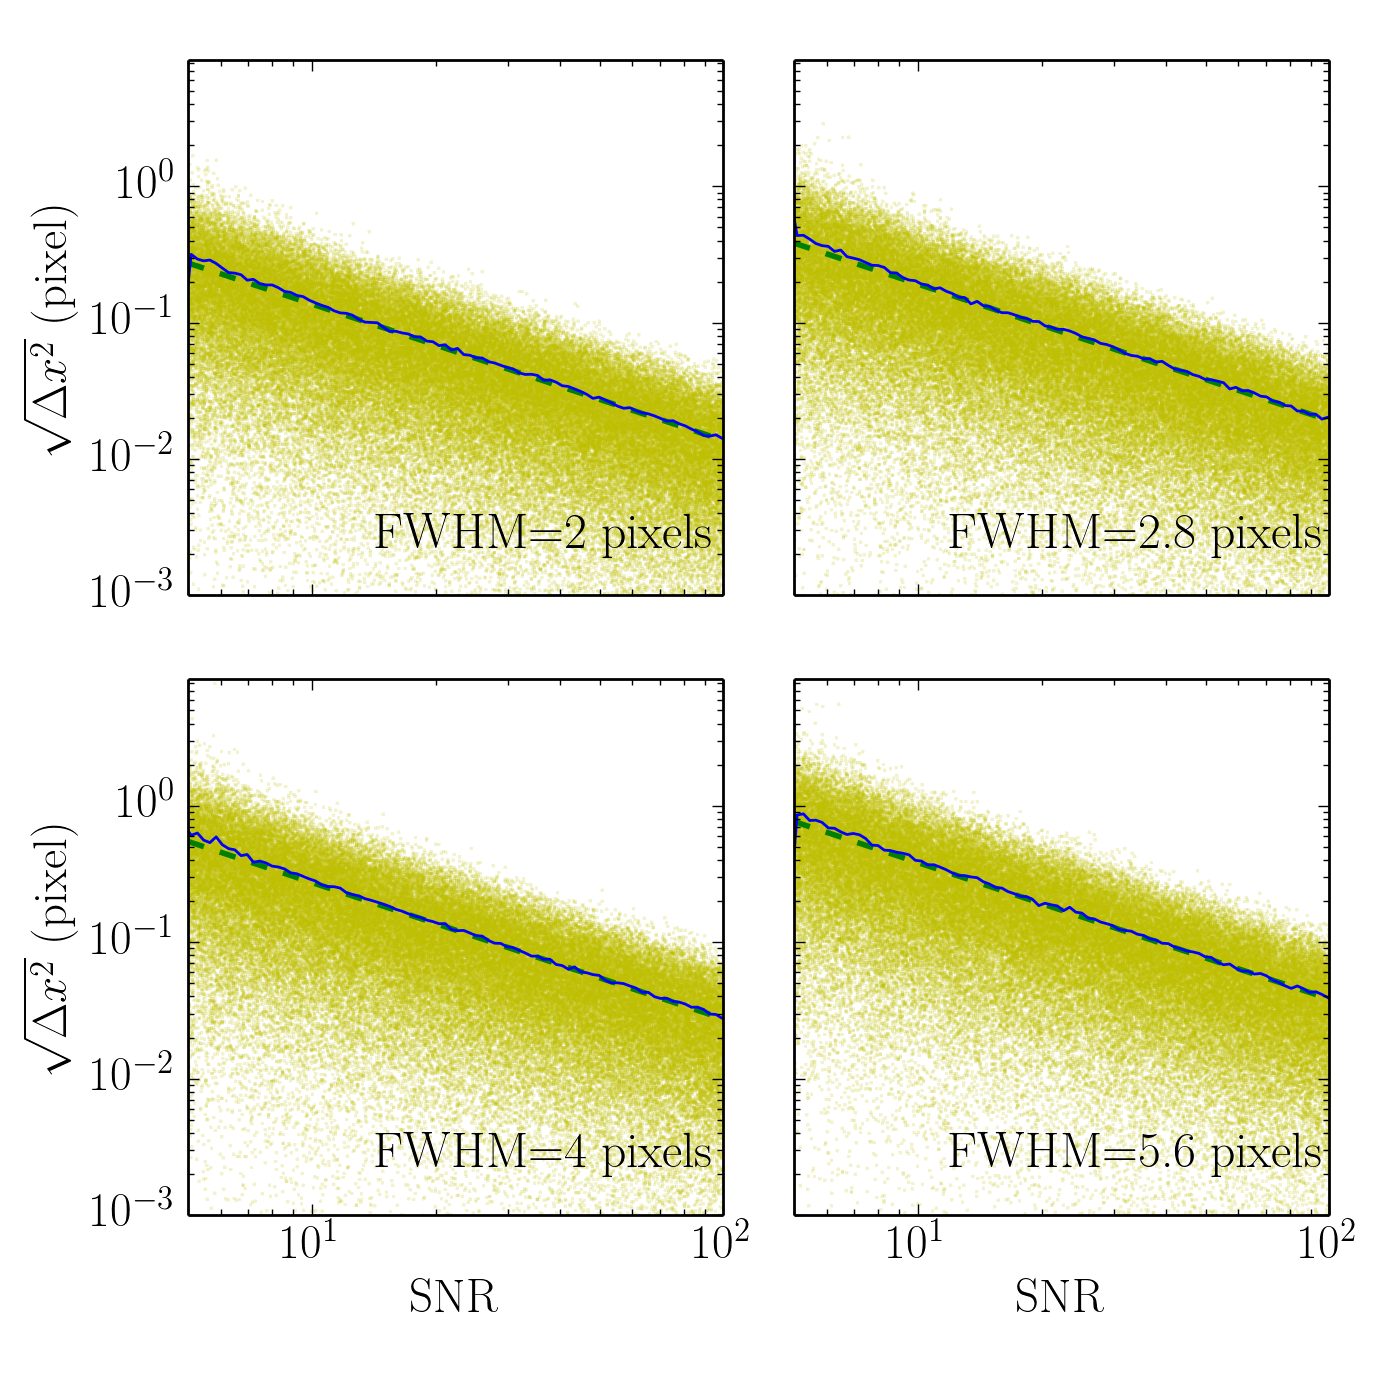
\includegraphics[width=\linewidth]{snr_psffitting.png}
\endminipage
\caption{Scatter plots showing the relation between error in centroid measurement
from fitting the exact PSF model to the stars and the signal-to-noise ratio of stars,
with FWHM of : 2 (upper left), 2.8 (upper right), 4 (lower left), and 5.6 (lower right)
pixels. In each scatter plot, the blue solid line represents the root-mean-squared-error, and the green dashed line represents CRLB.}\label{1}
\end{figure}

\begin{figure}[!htb]
\minipage{.8\textwidth}
  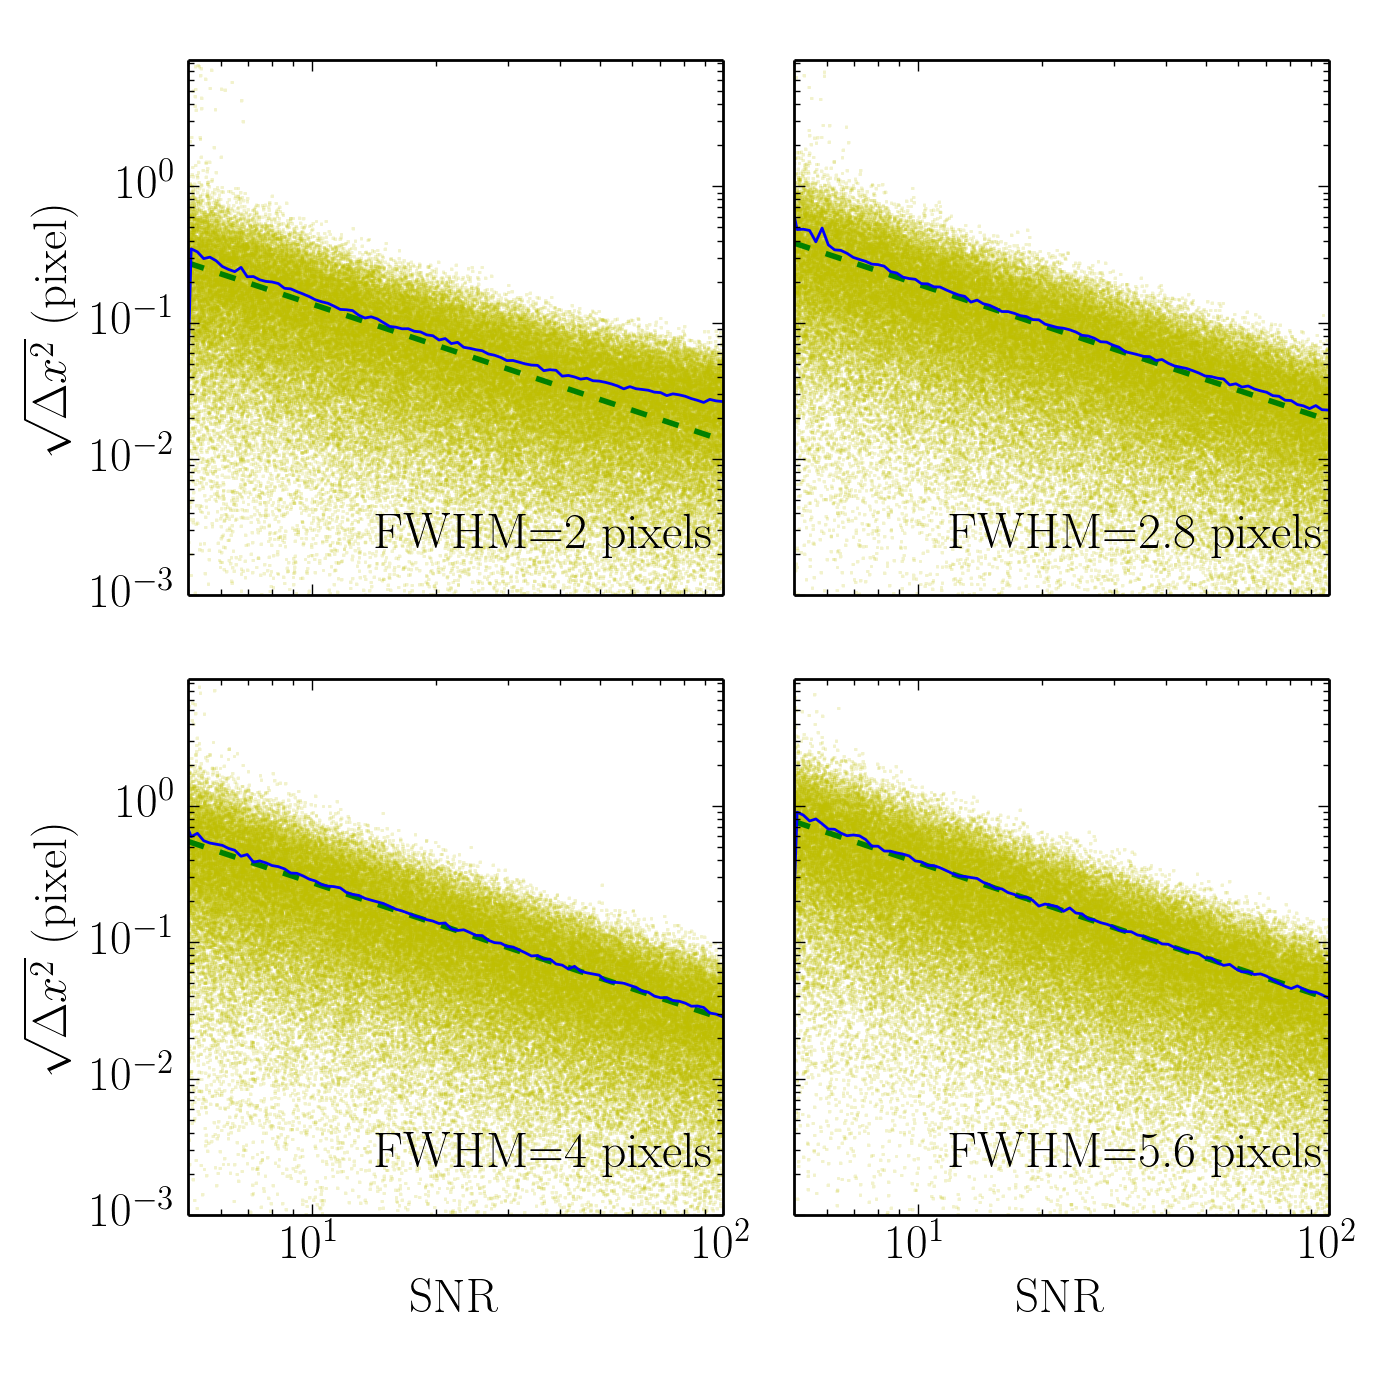
\includegraphics[width=\linewidth]{snr_psfpoly.png}
\endminipage
\caption{Scatter plots showing the relation between error in centroid
measurement from the PSF-based 3$\times$3 polynomial method and the signal-to-noise
ratio of stars, with FWHM of : 2 (upper left), 2.8 (upper right), 4 (lower left),
and 5.6 (lower right) pixels. In each scatter plot, the blue solid line represents the root-mean-squared-error, and the green dashed line represents CRLB.}\label{2}
\end{figure}

\begin{figure}[!htb]
\minipage{.8\textwidth}
  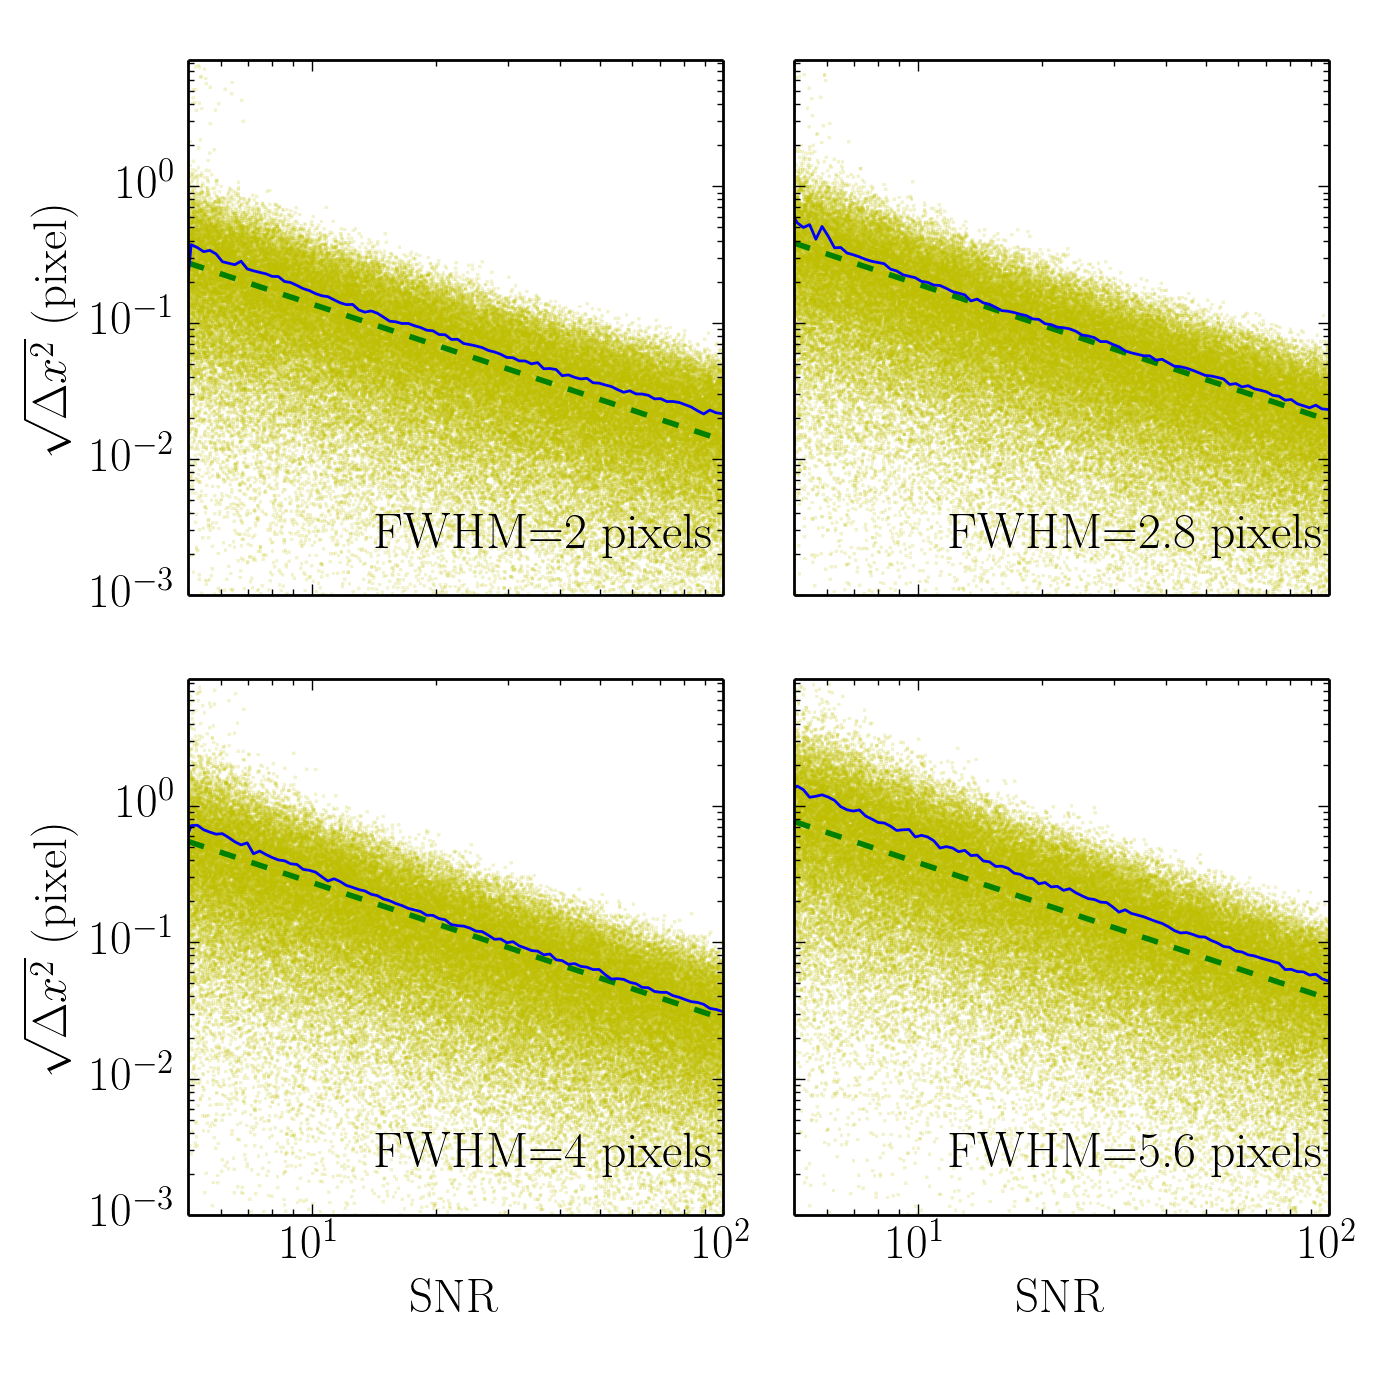
\includegraphics[width=\linewidth]{snr_psfpix28poly.png}
\endminipage
\caption{Scatter plots showing the relation between error in centroid measurement from the 3$\times$3 polynomial centroiding and the signal-to-noise ratio of stars, with FWHM of : 2 (upper left), 2.8 (upper right), 4 (lower left), and 5.6 (lower right) pixels. In each scatter plot, the blue solid line represents the root-mean-squared-error, and the green dashed line represents CRLB.}\label{3}
\end{figure}

\begin{figure}[!htb]
\minipage{.8\textwidth}
  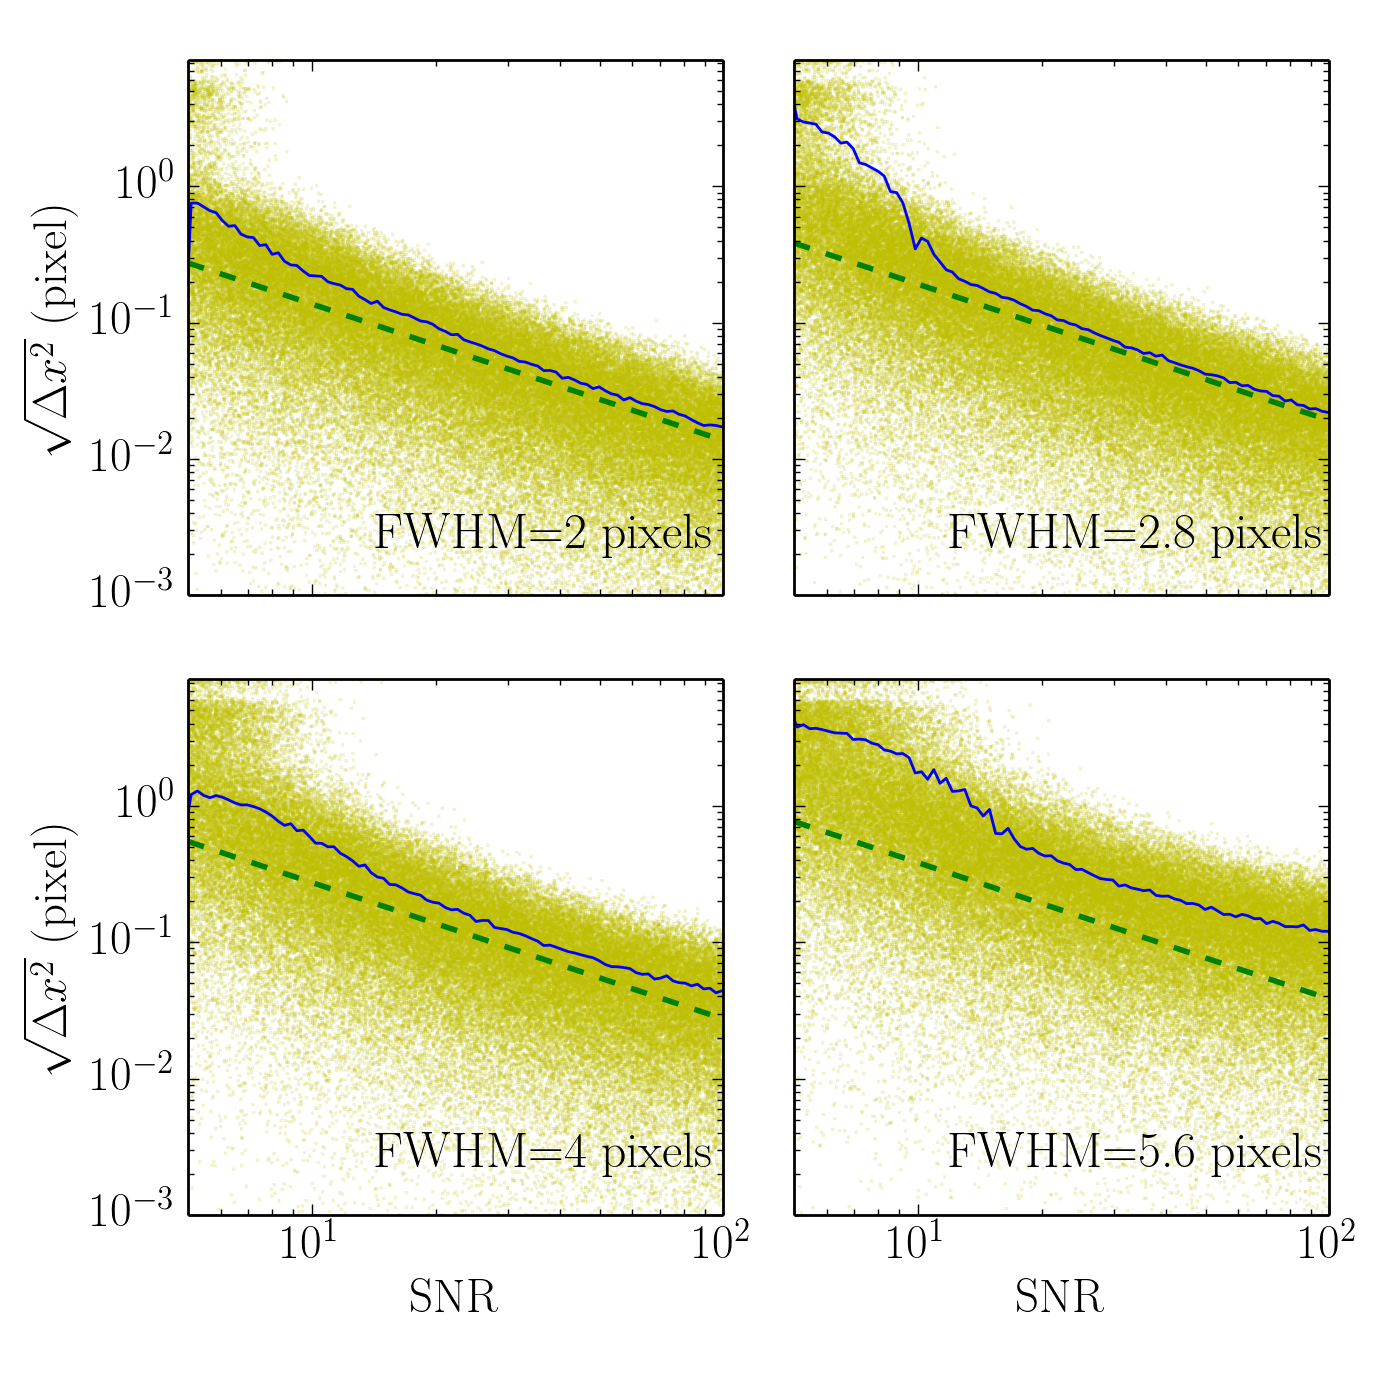
\includegraphics[width=\linewidth]{snr_moment.png}
\endminipage
\caption{Scatter plots showing the relation between error in centroid measurement from the 7$\times$7 moment method and the signal-to-noise ratio of stars, with FWHM of : 2 (upper left), 2.8 (upper right), 4 (lower left), and 5.6 (lower right) pixels. In each scatter plot, the blue solid line represents the root-mean-squared-error, and the green dashed line represents CRLB.}\label{4}
\end{figure}

%%%%%%%%%%%%%%%%%%%%%%%%%%%%%%%%%%%%%%%%%%%%%%%%%%%%%%%%%%%%%%%%%%%%%%%%%%% FWHM PLOTS %%%%%%%%%%%%%%%%%%%%%%%%%%%%%%%%%%%%%%%%%%

\begin{figure}[!htb]
\minipage{.8\textwidth}
  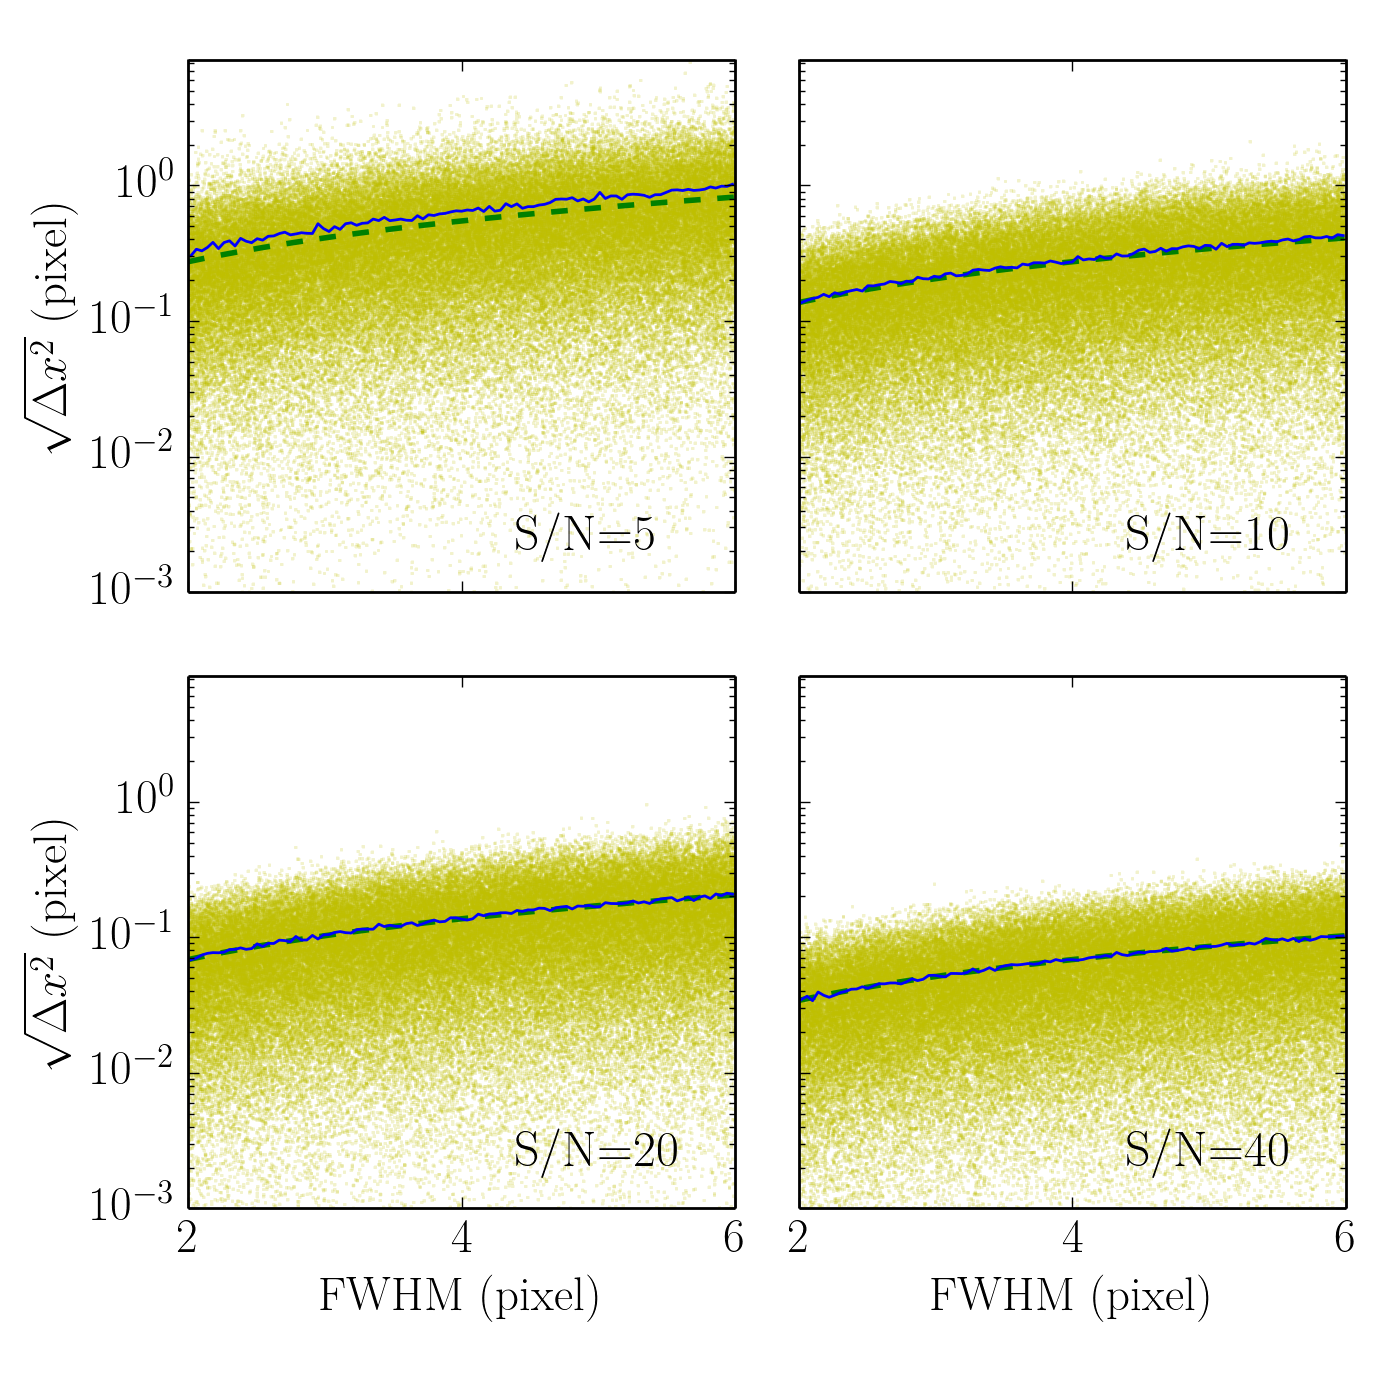
\includegraphics[width=\linewidth]{fwhm_psf.png}
\endminipage
\caption{Scatter plots showing the relation between error in centroid measurement
from fitting the exact PSF model and FWHM of stars, with SNR  of : 5 (upper left),
10 (upper right), 20 (lower left), and 40 (lower right). In each scatter plot,
the blue solid
 line represents the root-mean-squared-error, and the green dashed line represents CRLB.}\label{5}
\end{figure}

\begin{figure}[!htb]
\minipage{.8\textwidth}
  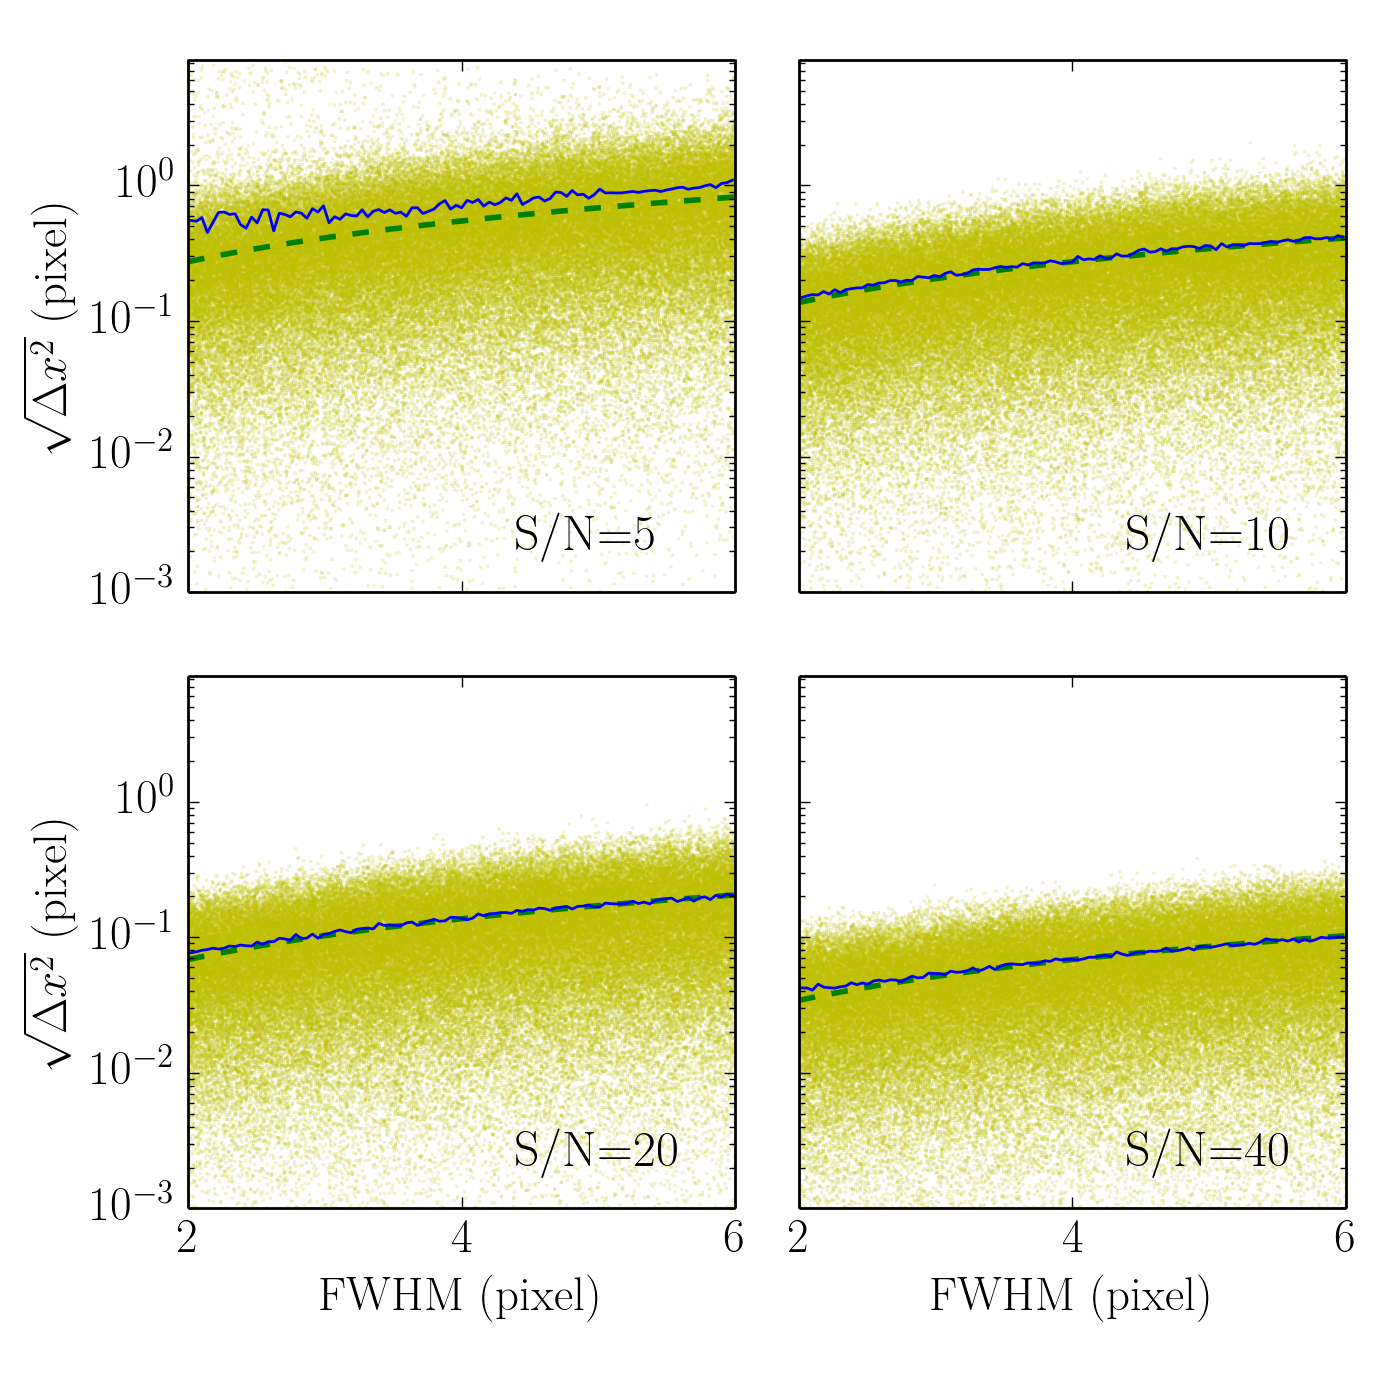
\includegraphics[width=\linewidth]{fwhm_psfpoly.png}
\endminipage
\caption{Scatter plots showing the relation between error in centroid measurement
from the PSF-based 3$\times$3 polynomial method and FWHM of stars, with SNR  of : 5 (upper left),
10 (upper right), 20 (lower left), and 40 (lower right). In each scatter plot, the blue solid
 line represents the root-mean-squared-error, and the green dashed line represents CRLB.}\label{6}
\end{figure}

\begin{figure}[!htb]
\minipage{.8\textwidth}
  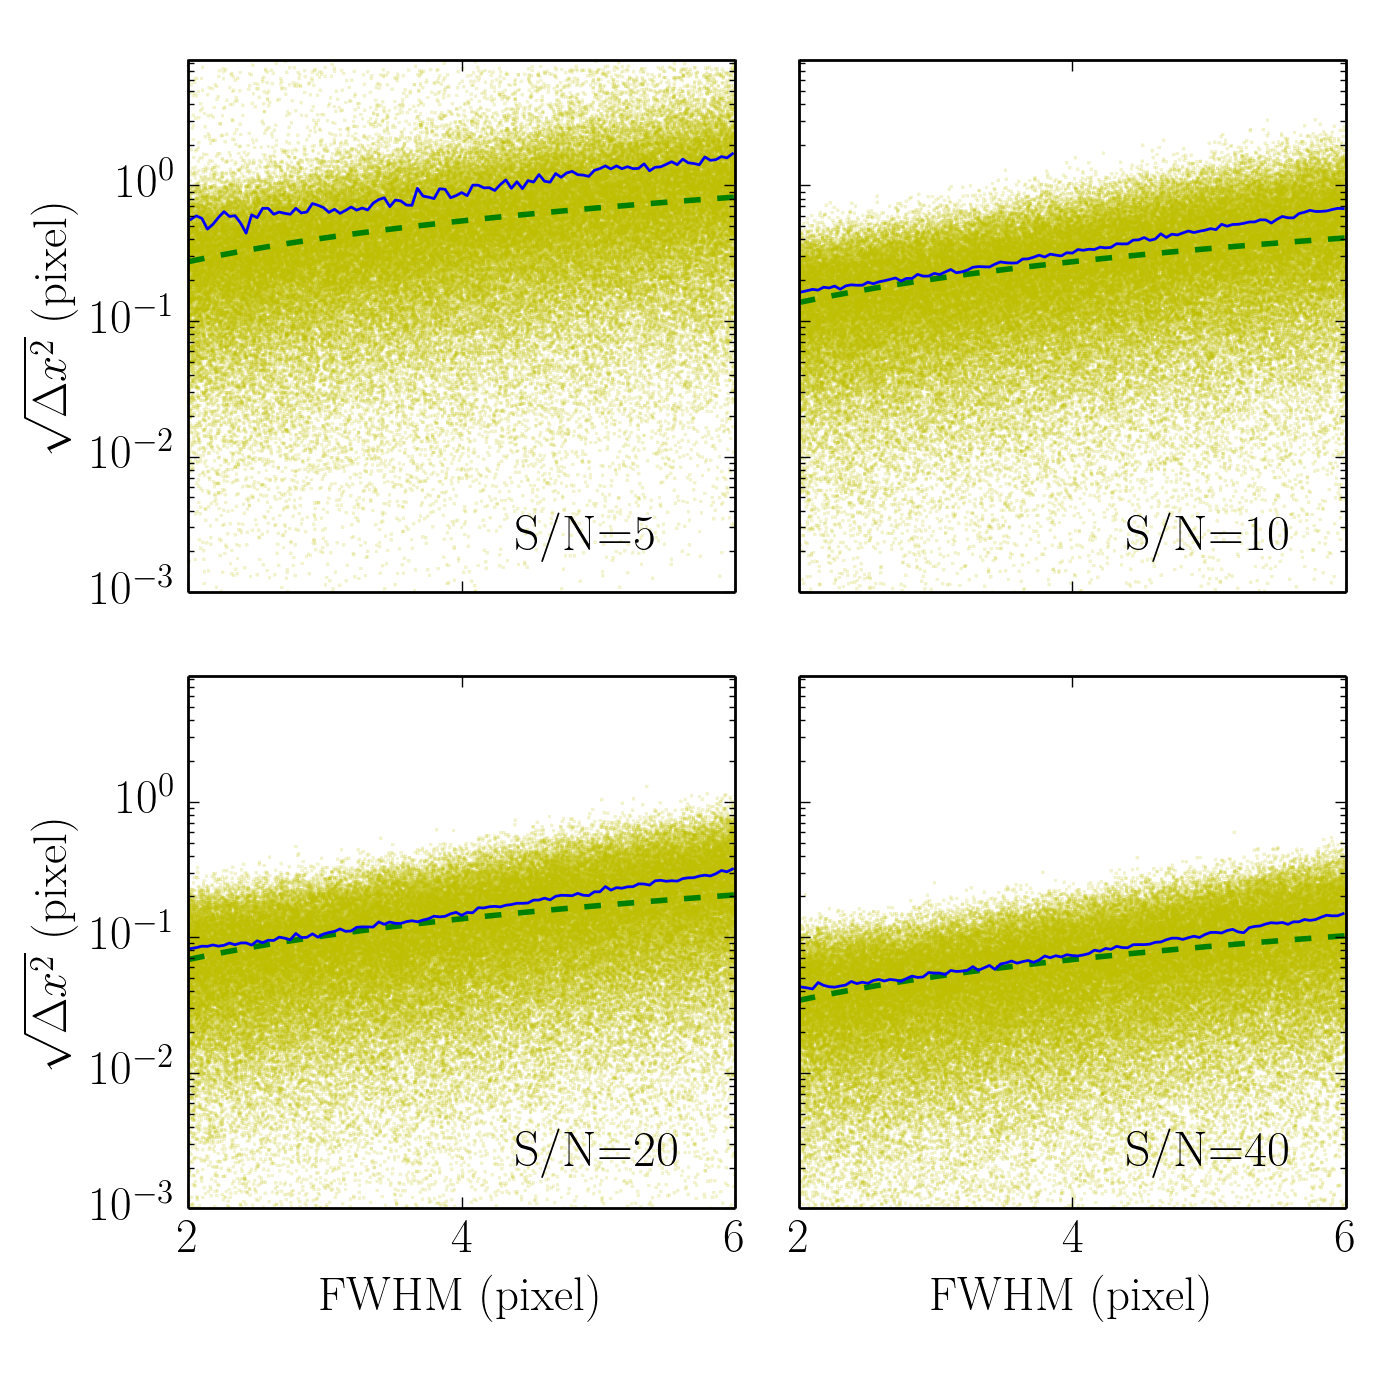
\includegraphics[width=\linewidth]{fwhm_psfpix28poly.png}
\endminipage
\caption{Scatter plots showing the relation between error in centroid measurement
from the 3$\times$3 polynomial centroiding and FWHM of stars, with SNR  of 
: 5 (upper left), 10 (upper right), 20 (lower left), and 40 (lower right). In each
scatter plot, the blue solid
 line represents the root-mean-squared-error, and the green dashed line represents CRLB.}\label{7}
\end{figure}

\begin{figure}[!htb]
\minipage{.8\textwidth}
  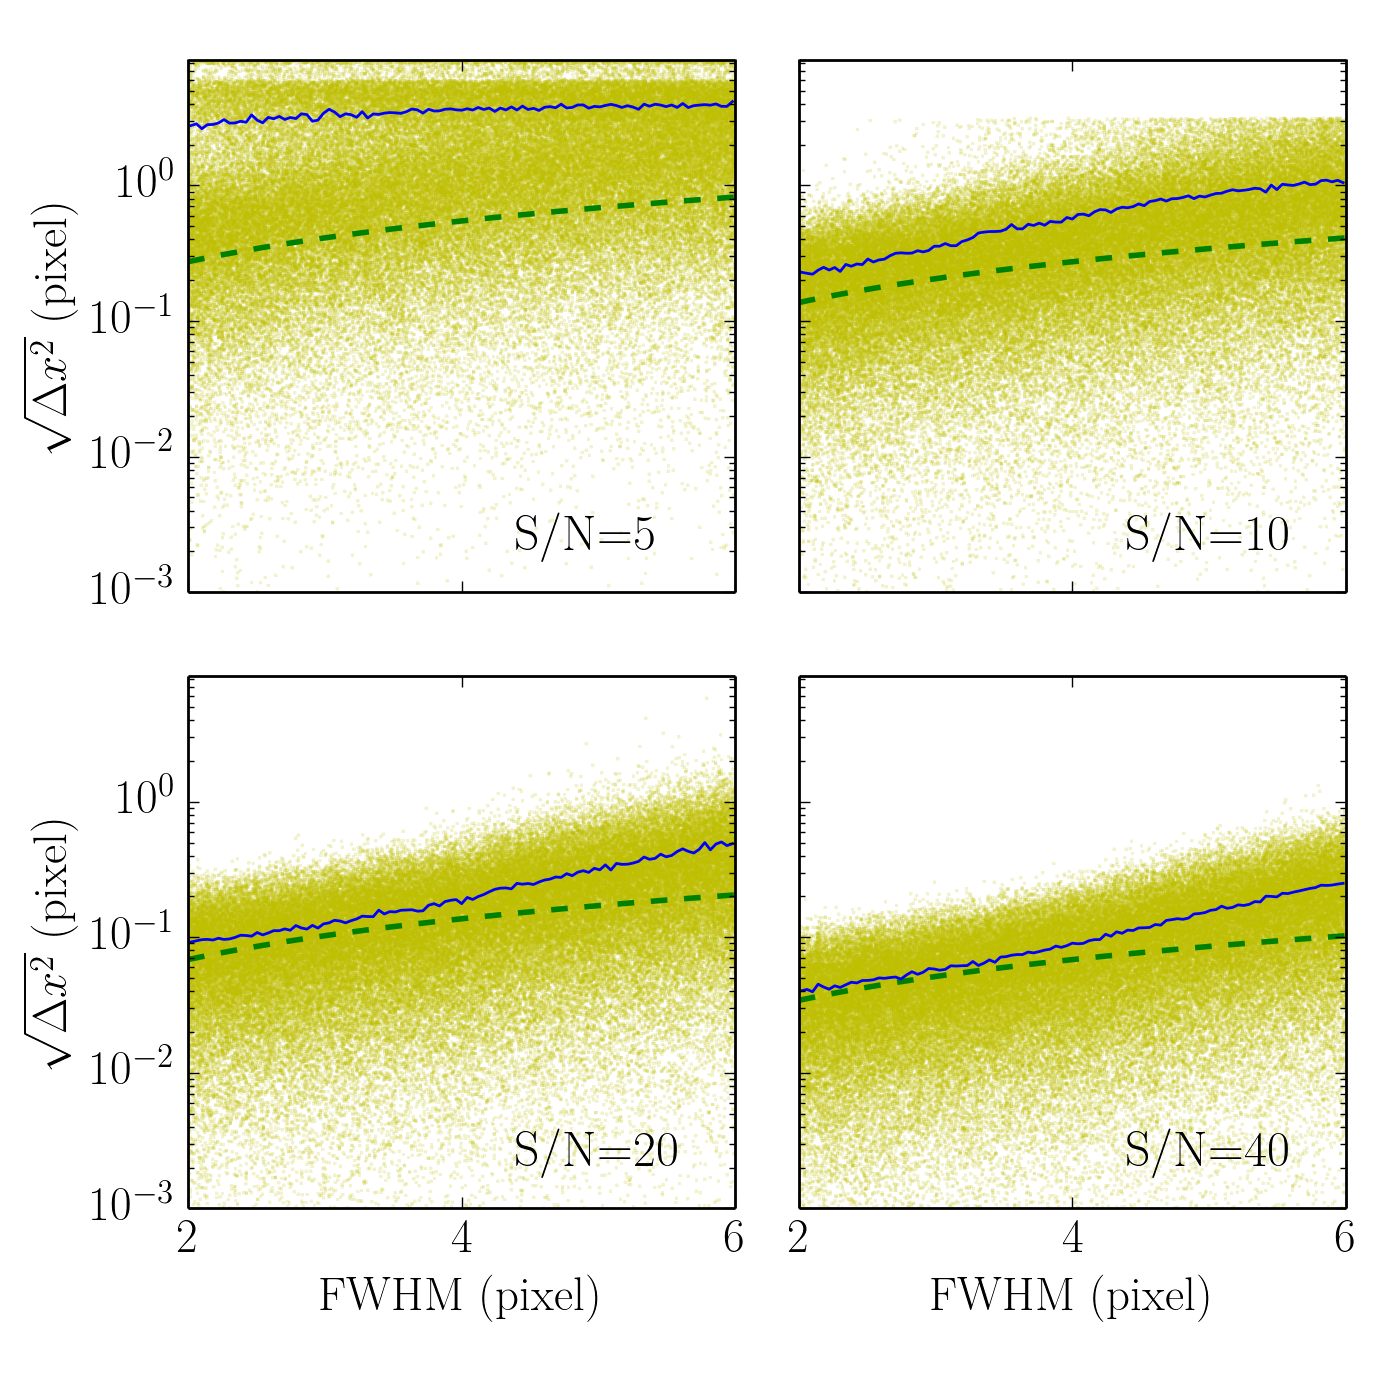
\includegraphics[width=\linewidth]{fwhm_moment.png}
\endminipage
\caption{Scatter plots showing the relation between error in centroid measurement
from the 7$\times$7 moment method and FWHM of stars, with SNR of : 5 (upper left),
10 (upper right), 20 (lower left), and 40 (lower right). In each scatter plot, 
the blue solid
 line represents the root-mean-squared-error, and the green dashed line represents CRLB.}\label{8}
\end{figure}

\end{document}
